\documentclass{beamer}
\usepackage[utf8]{inputenc}

\usetheme{Madrid}
\usecolortheme{default}
\usepackage{amsmath,amssymb,amsfonts,amsthm}
\usepackage{mathtools}
\usepackage{txfonts}
\usepackage{tkz-euclide}
\usepackage{listings}
\usepackage{adjustbox}
\usepackage{tfrupee}
\usepackage{array}
\usepackage{gensymb}
\usepackage{tabularx}
\usepackage{gvv}
\usepackage{lmodern}
\usepackage{circuitikz}
\usepackage{tikz}
\lstset{literate={·}{{$\cdot$}}1 {λ}{{$\lambda$}}1 {→}{{$\to$}}1}
\usepackage{graphicx}

\setbeamertemplate{page number in head/foot}[totalframenumber]

\usepackage{tcolorbox}
\tcbuselibrary{minted,breakable,xparse,skins}

\definecolor{bg}{gray}{0.95}
\DeclareTCBListing{mintedbox}{O{}m!O{}}{%
  breakable=true,
  listing engine=minted,
  listing only,
  minted language=#2,
  minted style=default,
  minted options={%
    linenos,
    gobble=0,
    breaklines=true,
    breakafter=,,
    fontsize=\small,
    numbersep=8pt,
    #1},
  boxsep=0pt,
  left skip=0pt,
  right skip=0pt,
  left=25pt,
  right=0pt,
  top=3pt,
  bottom=3pt,
  arc=5pt,
  leftrule=0pt,
  rightrule=0pt,
  bottomrule=2pt,
  toprule=2pt,
  colback=bg,
  colframe=orange!70,
  enhanced,
  overlay={%
    \begin{tcbclipinterior}
    \fill[orange!20!white] (frame.south west) rectangle ([xshift=20pt]frame.north west);
    \end{tcbclipinterior}},
  #3,
}
\lstset{
    language=C,
    basicstyle=\ttfamily\small,
    keywordstyle=\color{blue},
    stringstyle=\color{orange},
    commentstyle=\color{green!60!black},
    numbers=left,
    numberstyle=\tiny\color{gray},
    breaklines=true,
    showstringspaces=false,
}

\title{9.4.25}
\date{September 22, 2025}
\author{Bhargav - EE25BTECH11013}

\begin{document}

\frame{\titlepage}

\begin{frame}{Question}
\textbf{Question}: \\
Find the roots of the quadratic equation graphically.
\begin{align}
5x^2 - 6x - 2 = 0
\end{align}
\end{frame}

\begin{frame}{Solution}
\begin{align}
y = 5x^2 - 6x - 2 = 0
\end{align}

This equation can be represented as the conic
\begin{align}
\vec{x^T}\vec{V}\vec{x} + 2\vec{u^T}\vec{x} + f = 0
\end{align}
\begin{align}
\vec{V} = \myvec{5 & 0 \\ 0 & 0}, \vec{u} = \myvec{-3 \\ 0}, f = -2
\end{align}
\end{frame}

\begin{frame}{Solution}
To find the roots, we find the points of intersection of the conic with the x-axis.
\begin{align}
\vec{x} = \vec{h} + k_i\vec{m}    
\end{align}
\begin{align}
\vec{h}=\myvec{0 \\ 0}, \vec{m} = \myvec{1 \\ 0}
\end{align}
\end{frame}

\begin{frame}{Solution}
The value of $k_i$ can be found out by solving the line and conic equation
\begin{align}
(\vec{h} + k_i \vec{m})^{\top} \vec{V} (\vec{h} + k_i \vec{m}) + 2\vec{u}^{\top} (\vec{h} + k_i \vec{m}) + f &= 0 \\
\implies k_i^{2} \vec{m}^{\top}\vec{V}\vec{m} + 2k_i \vec{m}^{\top} (\vec{V}\vec{h} + \vec{u}) + \vec{h}^{\top}\vec{V}\vec{h} + 2\vec{u}^{\top}\vec{h} + f &= 0 \\
\text{or, } k_i^{2} \vec{m}^{\top}\vec{V}\vec{m} + 2k_i \vec{m}^{\top} (\vec{V}\vec{h} + \vec{u}) + g(\vec{h}) &= 0
\end{align}
\end{frame}

\begin{frame}{Solution}
Solving the above quadratic gives the equation
\begin{align}
k_i = \frac{1}{\vec{m}^{\top}\vec{V}\vec{m}}
\brak{
    -\vec{m}^{\top} (\vec{V}\vec{h} + \vec{u})
    \;\pm\;
    \sqrt{ \sbrak{\vec{m}^{\top}(\vec{V}\vec{h} + \vec{u})}^2
    - g(\vec{h}) \, (\vec{m}^{\top}\vec{V}\vec{m}) }
    }
\end{align}

\begin{align}
\therefore k_i = \frac{3}{5} \;\pm\; \frac{\sqrt{19}}{5}
\end{align}
\end{frame}

\begin{frame}{Solution}
\begin{align}
\implies k_1 = \frac{3}{5} + \frac{\sqrt{19}}{5}, \quad k_2 = \frac{3}{5} - \frac{\sqrt{19}}{5}
\end{align}

\begin{align}
\therefore \vec{x} = \vec{h} + k_i\vec{m} = \myvec{\frac{3}{5} + \frac{\sqrt{19}}{5} \\ 0} ,  \myvec{\frac{3}{5} - \frac{\sqrt{19}}{5} \\ 0}
\end{align}

\end{frame}

\begin{frame}{Plot}
\begin{figure}[h!]
    \centering
    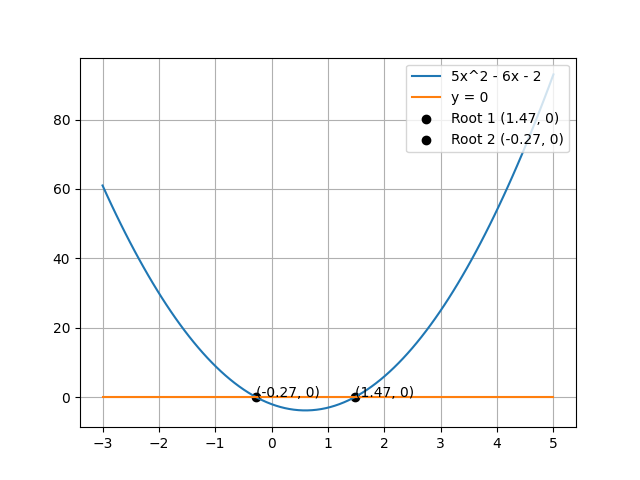
\includegraphics[height=0.5\textheight, keepaspectratio]{figs/Figure_1.png}
    \label{figure_1}
\end{figure}
\end{frame}

\begin{frame}[fragile]
    \frametitle{C Code}
    \begin{lstlisting}
#include <stdio.h>
#include <math.h>

double root1(double a, double b, double c) {
    double d = b*b - 4*a*c;
    return (-b + sqrt(d)) / (2*a);
}

double root2(double a, double b, double c) {
    double d = b*b - 4*a*c;
    return (-b - sqrt(d)) / (2*a);
}





    \end{lstlisting}
\end{frame}
\begin{frame}[fragile]
    \frametitle{Python + C Code}
    \begin{lstlisting}
import numpy as np
import matplotlib.pyplot as plt
import ctypes
lib = ctypes.CDLL("./libcode.so")
lib.root1.argtypes = [ctypes.c_double, ctypes.c_double, ctypes.c_double]
lib.root1.restype = ctypes.c_double
lib.root2.argtypes = [ctypes.c_double, ctypes.c_double, ctypes.c_double]
lib.root2.restype = ctypes.c_double
def quadratic(a, b, c):
    x1 = lib.root1(a, b, c)
    x2 = lib.root2(a, b, c)
    return x1, x2
def function(x):
    return 5*(x**2) - 6*x - 2
x = np.linspace(-3, 5, 100)
y = function(x)


    \end{lstlisting}
\end{frame}
\begin{frame}[fragile]
    \frametitle{Python + C Code}
    \begin{lstlisting}
y1 = np.zeros(100)
x1, x2 = quadratic(5, -6, -2)
fig, ax = plt.subplots()
ax.plot(x, y, label='5x^2 - 6x - 2')
ax.plot(x, y1, label='y = 0')
ax.scatter(x1, 0, color="black", label=f'Root 1 ({x1:.2f}, 0)')
ax.text(x1, 0, f'({x1:.2f}, 0)')
ax.scatter(x2, 0, color="black", label=f'Root 2 ({x2:.2f}, 0)')
ax.text(x2, 0, f'({x2:.2f}, 0)')
ax.grid(True)
ax.legend(loc="upper right")
plt.savefig("/Users/bhargavkrish/Desktop/BackupMatrix/ee25btech11013/matgeo/9.4.25/figs/Figure_1.png")
plt.show()



    \end{lstlisting}
\end{frame}
\begin{frame}[fragile]
    \frametitle{Python Code}
    \begin{lstlisting}
import numpy as np
import matplotlib.pyplot as plt
def function(x):
  return 5*(x**2) - 6*x - 2;
x = np.linspace(-3, 5, 100)
y = function(x)
y1 = np.zeros(100)
def quadratic(a, b, c):
  d = b**2 - 4*a*c
  x1 = (-b + np.sqrt(d)) / (2*a)
  x2 = (-b - np.sqrt(d)) / (2*a)
  return x1, x2

x1, x2 = quadratic(5, -6, -2)
fig, ax = plt.subplots()
ax.plot(x, y, label='5x^2 - 6x - 2') 
ax.plot(x, y1, label='y = 0') 

    \end{lstlisting}
\end{frame}

\begin{frame}[fragile]
    \frametitle{Python Code}
    \begin{lstlisting}
ax.scatter(x1, 0, color="black", label=f'Root 1 ({x1:.2f}, 0)') 
ax.text(x1, 0, f'({x1:.2f}, 0)')
ax.scatter(x2, 0, color="black", label=f'Root 2 ({x2:.2f}, 0)') 
ax.text(x2, 0, f'({x2:.2f}, 0)')
ax.grid(True)
ax.legend() 
ax.legend(loc="upper right")
plt.savefig("/Users/bhargavkrish/Desktop/BackupMatrix/ee25btech11013/matgeo/9.4.25/figs/Figure_1.png")
plt.show()


    \end{lstlisting}
\end{frame}
\end{document}

